\section{Comparative Evaluation and Design Decisions}
\label{sec:comparisons}
The comparisons ask which changes improve a specific software boundary.
A \emph{case} is one input, its permitted evidence and expected behaviour;
a \emph{history} contains many dependent turns for a simulated learner.
An \emph{arm} is one tested configuration. A \emph{gate} is a required acceptance condition, so a high average cannot
compensate for a critical error. The comparison names below link to exact records in
Appendix~\ref{sec:study-index}.

\begin{table}[htbp]
\centering\small
\caption{Evaluation questions, configurations and case counts.}
\label{tab:evaluation-design}
\begin{tabularx}{\linewidth}{@{}L{0.29\linewidth}Y L{0.13\linewidth}@{}}
\toprule Comparison & Cases / separation & External LLM \\\midrule
Evidence-interface comparison & 497 development cases; three extractive architectures on the same fold & No \\
Fresh factual comparison & 1,000 fresh cases; five configurations fixed before evaluation, disjoint source families & No \\
Action-planning comparison & 1,000 synthetic contexts; two configurations; 2,000 context--configuration pairs & Yes \\
Model-allocation comparison & 300 contexts; four allocations; 1,200 context--configuration pairs & Yes \\
Learner/timing simulation & 240 simulated learners per condition; nine combinations and two bounds; 30 virtual days & No \\
Revision comparison & 56 fresh scenario pairs per candidate; adequate and defective drafts & Yes \\
Live-model integration trial & 24 synthetic histories, 30 virtual days; diagnostic output review & Yes \\
Goal-completion regression & 72 histories per arm; matched seeds, exposed six-concept fixture & No \\
\bottomrule
\end{tabularx}
\end{table}

Studies use synthetic or permitted material. Only configurations within the same study
are compared directly, with shared inputs and scoring. Sample grids provide
boundary and scenario coverage. The \hyperref[study-E]{learner/timing simulation} holds out seeds within its simulator assumptions;
the \hyperref[study-H]{goal-completion regression} is a targeted regression comparison on previously exposed concepts.

\subsection{Making Retrieved Evidence Usable by the Answer Generator}
\label{sec:grounding-comparison}
\textbf{Problem and alternatives.}
A question can require two facts although its highest-ranking passage contains
only one. The evidence contract therefore needs to identify both the target
and the number of required claims. Here, an any-hit gate accepts any retrieved
passage; the typed target/cardinality interface identifies the kind and number
of facts the question requires. The \hyperref[study-A]{evidence-interface comparison} compares a lexical/any-hit control,
a typed target-and-cardinality interface, and that interface with additional
section ranking. It freezes 397 answerable and 100 boundary cases; candidate
outputs were stored before opening hidden reference answers.

\begin{table}[htbp]
\centering\small
\caption{The \hyperref[study-A]{evidence-interface comparison}: changing the evidence-to-answer contract on one development fold.}
\label{tab:evidence-interface}
\begin{tabularx}{\linewidth}{@{}Yrrr@{}}
\toprule Architecture & Grounded answers & Complete evidence@3 & Boundary action \\\midrule
Lexical/any-hit & 253/397 (63.73\%) & 95.97\% & 100/100 \\
Question type + fact count & 355/397 (89.42\%) & 98.74\% & 100/100 \\
Typed target + section ranking & 355/397 (89.42\%) & 98.74\% & 100/100 \\
\bottomrule
\end{tabularx}
\end{table}

\textbf{Interpretation and decision.}
The typed contract improved grounded success by 25.69 percentage points;
multi-evidence success rose from zero to 90.20\%. Section ranking added no
quality improvement. Remaining failures included unresolved paraphrased targets,
neighbouring source regions and extracted claims that missed the required span.
The typed interface was retained as the next development baseline, with
\emph{Refine} status: no arm passed every quality gate. 

\paragraph{How factual success is scored.}
For answerable case $i$, $g_i=1$ requires the correct answer action, all required
answer spans, exact claim/citation coverage, valid source versions and no
operational failure. Otherwise $g_i=0$. Claim/citation precision and recall must
both equal one. For boundary case $j$, $b_j=1$ requires the expected
clarification, abstention or refusal action. In the \hyperref[study-B]{fresh factual comparison},
\begin{equation}
\begin{aligned}
\text{Grounded success}&=\frac{100}{N_A}\sum_i g_i
 =100\frac{506}{800}=63.25\%,\\
\text{Boundary accuracy}&=\frac{100}{N_B}\sum_j b_j
 =100\frac{192}{200}=96\%.
\end{aligned}
\label{eq:grounded-score}
\end{equation}
Missing a required second fact fails the whole case. Normalized text and source-range matching
make the scorer inspectable but do not provide unrestricted semantic grading.

Let $E_i$ be the required evidence items and $M_i(3)$ those matched within the
first three results under the source/version/range rules. Then
\begin{equation}
\text{Complete evidence@3}
=\frac{100}{N_A}\sum_i\mathbf{1}[M_i(3)=E_i].
\label{eq:retrieval-score}
\end{equation}
Retrieval can score one while an incomplete answer scores zero. The \hyperref[study-B]{fresh factual comparison}'s
retained BM25 configuration with the dominance gate retrieved complete evidence in 98\% of
answerable cases but delivered only 63.25\% fully grounded answers. Its
family-bootstrap 95\% interval was 58.75--67.63\%, resampling the 200 source
families 10,000 times rather than treating related questions as independent.
The hybrid arm with the same gate scored 62\%. BM25 was retained as the simpler local
fallback; both failed factual acceptance.

The \hyperref[study-B]{fresh factual comparison}'s any-hit control had zero cases satisfying the complete grounding rubric despite 98\% retrieval
coverage: it passed an unrestricted evidence set to a generator requiring one
or two selected claims. This incompatible composition differs from the \hyperref[study-A]{evidence-interface comparison}'s lexical
control. The dense/hybrid arms use the Qwen embedding model~\cite{qwen3-embedding-card}.

\subsection{What the 10,000-Case Tests Revealed}
\label{sec:large-regression}
The large tests answer a different question from the fresh 1,000-case comparison:
does a selected composition still behave correctly when a course contains many
potentially competing source regions? Three records must be distinguished. The pipeline-scale test's later correction is separately
indexed as \hyperref[study-L1c]{pipeline-test correction}.

\begin{table}[htbp]
\centering\small
\caption{Large-test evidence and its limits. The whole-corpus regression reuses the large product test's known corpus; it is
not fresh generalization evidence. A 1,000-case control is a subset comparison,
not an additional 1,000 independent questions.}
\label{tab:large-tests}
\begin{tabularx}{\linewidth}{@{}L{0.22\linewidth}L{0.24\linewidth}Y@{}}
\toprule Test & Execution unit & What the record supports \\ \midrule
\hyperref[study-L1]{pipeline-scale test} & 10,000 cumulative pipeline cases & Processing and validation completed. Later audit found that the authoring path saw the reference answer and supplied its answer/citation; it did not independently test product retrieval and generation. \\
\hyperref[study-L2]{large product test} & 10,000 product cases; 1,000 paired controls & 8,000 answerable and 2,000 boundary cases; product received the course and question before hidden scoring. Recorded 478 severe unsupported releases and 594 operational failures; release-quality gates failed. \\
\hyperref[study-L3]{whole-corpus regression} & Same known 10,000 cases; 1,000 paired controls & Deterministic ambiguity-checking candidate; no external LLM calls. Recorded four severe unsupported releases, zero operational failures and 6,973 clarifications. Eleven of sixteen gates failed. \\
\bottomrule
\end{tabularx}
\end{table}

The large product test reported pooled grounded success of 44.16\%. Its
hierarchical source-family estimate was 42.94\% (95\% interval
41.03--44.96\%); the interval belongs to that estimate, not the pooled rate.

\textbf{Failure mechanism.}
The original ambiguity gate compared distinct answer meanings across every candidate
above a coverage threshold. In a full course, a weaker region could therefore
compete with the strongest relevant answer. Earlier confirmation published only
one approved chunk per release, so this ambiguity branch could not fire.
Figure~\ref{fig:evidence-failure} explains why passing that confirmation did
not establish corpus-scale behaviour. The 100-case diagnostic found the target
region ranked first in 84 cases, with 69 of those still returning clarification.
This motivated comparing dominant interpretations rather than all weak matches.
The subsequent fresh factual comparison remains the evidence for the retained fallback;
its quality gates also failed.

\textbf{Unresolved numerical inconsistency.}
The whole-corpus regression's durable summary labels 25.38\% as fully grounded factual success over
8,000 answerable cases, but separately records only 1,669 answer actions in all
10,000 cases. Under the scorer's requirement of a correct answer action, the
upper bound from that action count is $1669/8000=20.86\%$. These fields cannot
both describe the same scored ledger. The original record is preserved; the
25.38\% value is excluded from performance comparisons pending reconciliation
with the original per-case ledger, which was not located in the inspected
local evidence. The failure diagnosis and recorded
gate dispositions are reported as such, without turning that percentage into
a validated accuracy claim.

\begin{figure}[htbp]
\centering
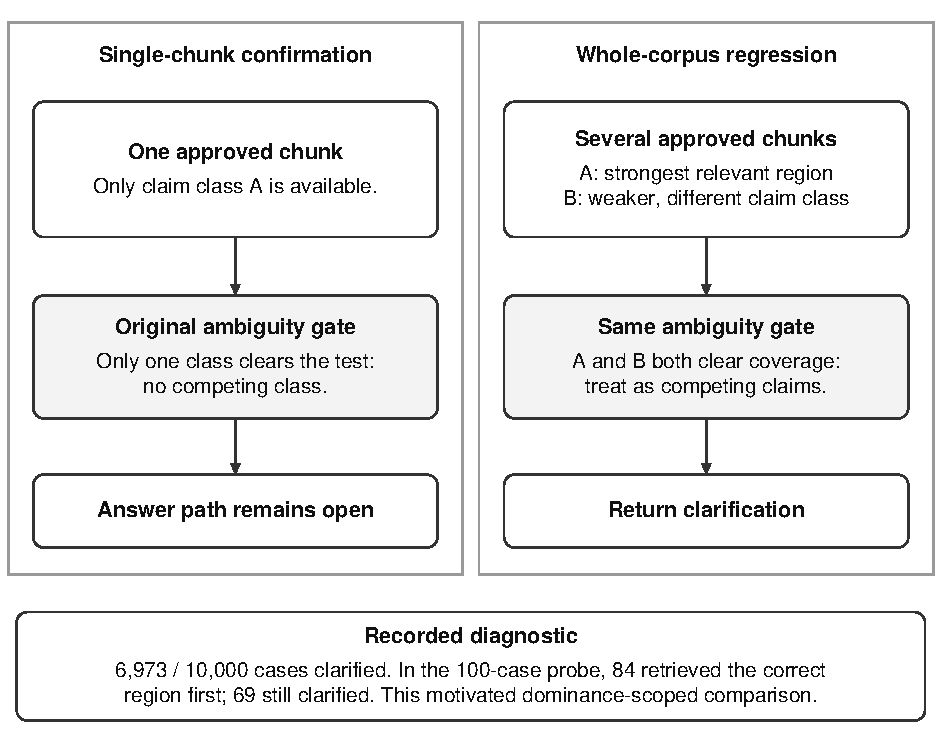
\includegraphics[width=\linewidth]{../../../reports/figures/course-twin-evidence-failure.pdf}
\caption{Original ambiguity checks under single-chunk and whole-corpus inputs (Whole-corpus regression).}
\label{fig:evidence-failure}
\end{figure}

\subsection{Selecting Actions and Allocating Models}
\label{sec:planner-comparison}
\textbf{Problem and alternatives.}
The planner must use model proposals without allowing malformed or unsuitable
proposals to suppress a valid baseline action. Earlier fixed-rule, model-only,
hierarchical and reject-only-verifier trials led to the guarded design.
The \hyperref[study-C]{action-planning comparison} then compared that design with the deterministic workflow on 1,000
synthetic contexts. These component trials supply explicit planning-state cards;
they do not validate the default product adapter's delivery-count proxy.

\begin{table}[htbp]
\centering\small
\caption{Action-planner results on 1,000 shared contexts.}
\label{tab:planner-comparison}
\begin{tabularx}{\linewidth}{@{}Yrrrr@{}}
\toprule Planner & Valid action & Preferred & Utility & Regret \\\midrule
Deterministic workflow & 100\% & 74\% & 0.7954 & 0.0129 \\
Guarded policy-value & 100\% & 73\% & 0.8002 & 0.0081 \\
\bottomrule
\end{tabularx}
\end{table}

Here, evaluation utility is the synthetic instrument's registered action value,
using the public state card and a seeded hidden learner outcome. For example,
not knowing the concept adds value to diagnostic support or a hint, and the
event type supplies an action-specific bonus. Mean regret is the difference
from the highest-valued permitted action.
Preferred-action agreement checks a separate reference label. Neither is
measured student learning, and this evaluation utility must not be confused
with the runtime heuristic $U$ in Equation~\ref{eq:planning-utility}.
The positive paired utility improvement replicated while hard gates held,
so the guarded planner advanced to engine comparison. Preferred agreement fell
by one percentage point; the result supports a conditional design choice,
not improvement on every definition of appropriate action.

The \hyperref[study-D]{model-allocation comparison} holds the architecture fixed and crosses two planner models with two
wording models. Table~\ref{tab:model-allocation} shows the complete four-way
comparison. The alternative planner's pooled utility effect was $+0.000354$
(95\% interval $0$--$0.001062$). The alternative wording model's valid-strategy
effect was $+0.00417$ ($0$--$0.01042$). Neither satisfied the preregistered rule requiring the entire interval to exceed zero. The Terra-planner/Luna-wording combination also missed the 99.5\% generator-completion gate
at 238/240 calls; its two failures used the deterministic fallback.

\begin{table}[htbp]
\centering\small
\caption{The \hyperref[study-D]{model-allocation comparison}: model allocation under one guarded architecture.
Luna and Terra denote GPT-5.6 variants; Mini is GPT-5.4 Mini (2026-03-17).}
\label{tab:model-allocation}
\begin{tabularx}{\linewidth}{@{}YYrr@{}}
\toprule Planner & Wording & Utility & Valid final wording \\\midrule
Luna & Luna & 0.7935 & 100\% \\
Terra & Luna & 0.7938 & 100\% \\
Luna & Mini & 0.7935 & 100\% \\
Terra & Mini & 0.7938 & 100\% \\
\bottomrule
\end{tabularx}
\end{table}

The Luna-planner/Luna-wording combination was the simplest and least expensive eligible allocation under the recorded
rule and advanced to whole-system confirmation. Valid final wording includes
fallback behaviour; it does not imply every provider call succeeded. 

\subsection{Combining Learner Estimation with Intervention Timing}
\label{sec:timing-comparison}
\textbf{Problem and alternatives.}
Sending fewer reminders can reduce waste while also removing useful practice.
The \hyperref[study-E]{learner/timing simulation} separates the estimate of need from the decision to intervene. It
crosses a count baseline, Bayesian Knowledge Tracing (BKT) and Performance
Factors Analysis (PFA) with constant, conditional and value-based timing.
BKT updates a latent knowledge estimate from observed performance
\cite{corbett1994knowledge}; PFA relates performance to prior successful and
unsuccessful practice~\cite{pavlik2009performance}. The local variants include forgetting/decay.

Figure~\ref{fig:simulation-design} shows the development/held-out split and
which information the candidates can observe. The simulation does not execute
text retrieval or generation. The two bounds locate the comparison between
never intervening and using simulator knowledge unavailable to the candidates.

\begin{figure}[htbp]
\centering
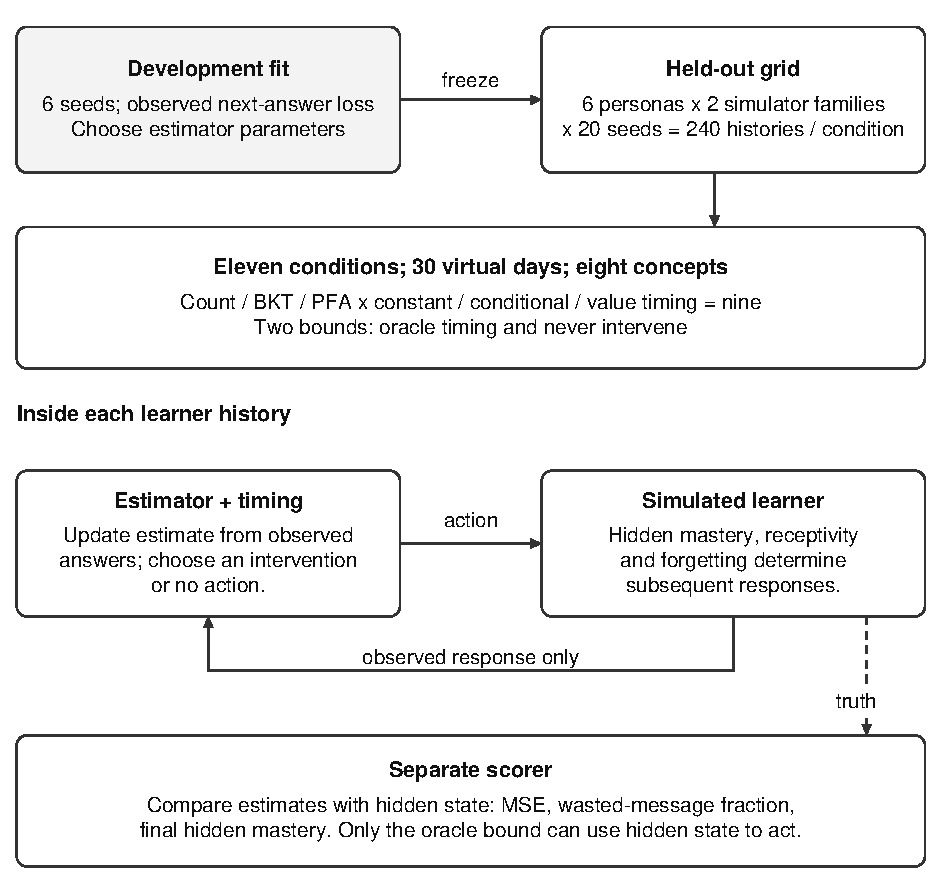
\includegraphics[width=\linewidth]{../../../reports/figures/course-twin-simulation-design.pdf}
\caption{Learner/timing simulation: held-out comparison with separate observation and scoring inputs.}
\label{fig:simulation-design}
\end{figure}

\begin{table}[htbp]
\centering\small
\caption{The \hyperref[study-E]{learner/timing simulation}: all nine estimator/timing combinations and two bounds.
Mean squared error (MSE) and waste are lower-is-better; mastery is a simulator state on $[0,1]$.
Messages and rates are means over 240 learners per condition.}
\label{tab:learner-timing}
\begin{tabularx}{\linewidth}{@{}Yrrrr@{}}
\toprule Estimator + timing & MSE & Messages & Waste & Final mastery \\\midrule
Count + constant (baseline) & 0.084 & 14.0 & 50.6\% & 0.314 \\
Count + conditional & 0.084 & 7.0 & 38.8\% & 0.302 \\
Count + value & 0.084 & 10.2 & 34.1\% & 0.317 \\
BKT + constant & 0.035 & 14.0 & 46.4\% & 0.317 \\
BKT + conditional & 0.035 & 8.9 & 36.6\% & 0.309 \\
BKT + value & 0.037 & 12.3 & 30.1\% & 0.328 \\
PFA + constant & 0.052 & 14.0 & 50.8\% & 0.313 \\
PFA + conditional & 0.051 & 7.3 & 41.5\% & 0.303 \\
PFA + value & 0.051 & 10.5 & 34.7\% & 0.313 \\\midrule
Count + oracle (bound) & 0.086 & 12.2 & 0.0\% & 0.345 \\
Count + never (bound) & 0.083 & 0.0 & -- & 0.288 \\
\bottomrule
\end{tabularx}
\end{table}

For daily concept estimate $\hat m_{hct}$ and simulator truth $m_{hct}$,
MSE averages $(\hat m_{hct}-m_{hct})^2$ over concept-days within each history
$h$, then across histories. A delivered intervention is labelled wasted when
the simulator says the learner is unreceptive or already has mastery at least
$0.85$. Waste is the mean of per-history wasted-delivery fractions, not a
human rating of the message. Final mastery averages hidden concept states on
day 30. The simulator defines all three quantities.

\begin{samepage}
\textbf{Interpretation and decision.}
BKT with value-based timing reduced waste by 20.5 percentage points relative
to count/constant (95\% paired-bootstrap interval $-22.8$ to $-18.3$ points).
Its final simulated mastery increased by $0.014$ ($0.007$--$0.021$), using
1,000 learner-level paired resamples. Count/conditional halved delivery but
reduced final mastery by $0.012$ ($-0.018$ to $-0.005$). Thus suppressing
messages alone did not deliver the best trade-off.
\end{samepage}

Hidden-state MSE improved, but BKT's next-answer Brier-score difference under
constant timing was inconclusive ($-0.00027$, 95\% interval $-0.00630$ to
$0.00552$). The initial attempt was invalidated because one
simulator's forgetting overwhelmed learning; its result and the corrected
attempt remain archived. The decision was \emph{Go Deeper}: retain BKT/value
as a hypothesis, with PFA as comparator. Integration with the product's
committed observations, a decayed-count control and a third simulator family
have not yet been completed. 

\subsection{Richer Instruction, Revision and Visual Evidence}
\textbf{Problem and alternatives.}
Constrained source assembly protects factual provenance but can produce generic
questions. Typed instructional units and bounded revision were evaluated to
allow more useful explanations while retaining source authority. A typed
instruction candidate was rated useful on 44/48 evaluated targets by assistant
review, compared with 16/48 for the control. These are rubric targets rather
than independent student judgments. The candidate retained one critical
attribution error. In the fresh \hyperref[study-F]{revision comparison}, each of two revision candidates received
56 adequate/defective scenario pairs. Both preserved 56/56 adequate drafts
and repaired 47/56 defective drafts (83.9\%), but each retained one critical
error. A cited necessary condition was treated as sufficient. Both failed
the zero-critical-error gate and remained unpromoted.

The reference answers were authored and cross-reviewed before candidate outputs were generated, and
uncertain judgments remained in the denominator. Nevertheless, the scoring
process was AI-assisted. Earlier source-oracle corrections and later response
audits that missed known critical errors show why structural validity and
citations do not establish semantic correctness. These failures are retained
alongside successful controls in the repository result records.

Visual experiments tested whether images supplied evidence that text lost.
In the historical comparison using the Jina embeddings v4 visual model~\cite{jina4-card}, relevant visual retrieval
improved from 18/30 to 28/30, yet both product arms achieved only 20/30 grounded
answers, and both retained critical citation failures. In a separate fresh comparison using the Jina embeddings v5 omni model~\cite{jina5-card},
the candidate achieved 16/30 grounded answers versus 26/30 for its text/OCR
control. Source-region lineage and packet layouts remained failure points;
the control also retained a citation defect. The omni candidate was dropped.
The selected product parser accepts selectable PDF text; general scanned-PDF
OCR remains unqualified.

